\documentclass[a4j,twocolumn,10pt]{jarticle}
\usepackage[dvipdfmx]{graphicx}
\usepackage{url}
\usepackage{color}
\usepackage[dvipdfmx]{hyperref}
\usepackage{pxjahyper}

\title{ミーティング資料}
\author{藤井敦寛}
\date{\today}


\begin{document}
\maketitle

\section{進捗状況}
DICOMO2020のテンプレに流して,再修正もしました.あとは,アイデア出しと先週のアイデアについて考えてました.

\section{今週のアイデア}
\begin{itemize}
  \item 特になし
\end{itemize}

\section{先週までのキープ案}
\begin{itemize}
  \item 乗り物乗車時の加速度センサのキャリブレーション

  ノイズ除去で探してみたが,特に類似してそうな論文は見つからなかった.

  電車乗車時などに,まず2秒間の加速度を取得しておく.この波形の周波数成分をノイズとして保存し,ジェスチャを行ったときの波形から減算する?

  \item 足の筋電から歩幅推定

  GPSから歩行距離がわかれば,距離/歩数で歩幅を得ることができる.歩数は筋電のピークから得られる.ただ,そもそも距離を得るのはOKなのか?

  少し論文を探してみましたが,関連1,2を見つけました.デッドレコニングという屋内歩行の位置推定を目的に歩幅推定を行うそうです.
  だとすると,距離を事前に得ることはNGかもしれません.でも,筋電の値のみでは歩幅推定は難しいような気がします.

  \item 歯の裏トラックパッド
\end{itemize}


\section{ボツ案}
\begin{itemize}
  \item 心電と脈波の時間差から個人識別
  \item 筋電による状態認識
  \item 物理フリックキーボード
  \item プロジェクターのスクリーンをタッチパネル化
  \item 警報音の目的判別
  \item あおり運転に繋がるドライバーの行動変化
  \item ドライバーの疲労度(腕の下がり)
  \item ライダーの疲労度変化(風圧,気温)
  \item グリップ内蔵型スイッチボックス
  \item 次世代型エンジンスタートシステム(ハンドル圧での認証,ドアノブ圧認証)
  \item 次世代型給油停止システム(センサ型)
  \item 人の歩幅を使った何か…疲労度とか?
  \item センサーで眼を観察して動きなどから視力低下限界警告
  \item 1km以上追越車線を走行した場合のアラートと,車線変更可能位置の誘導などの運転支援
  \item 硬筆文字のデジタル化
\end{itemize}

% \begin{figure*}[t]
%   \begin{center}
%     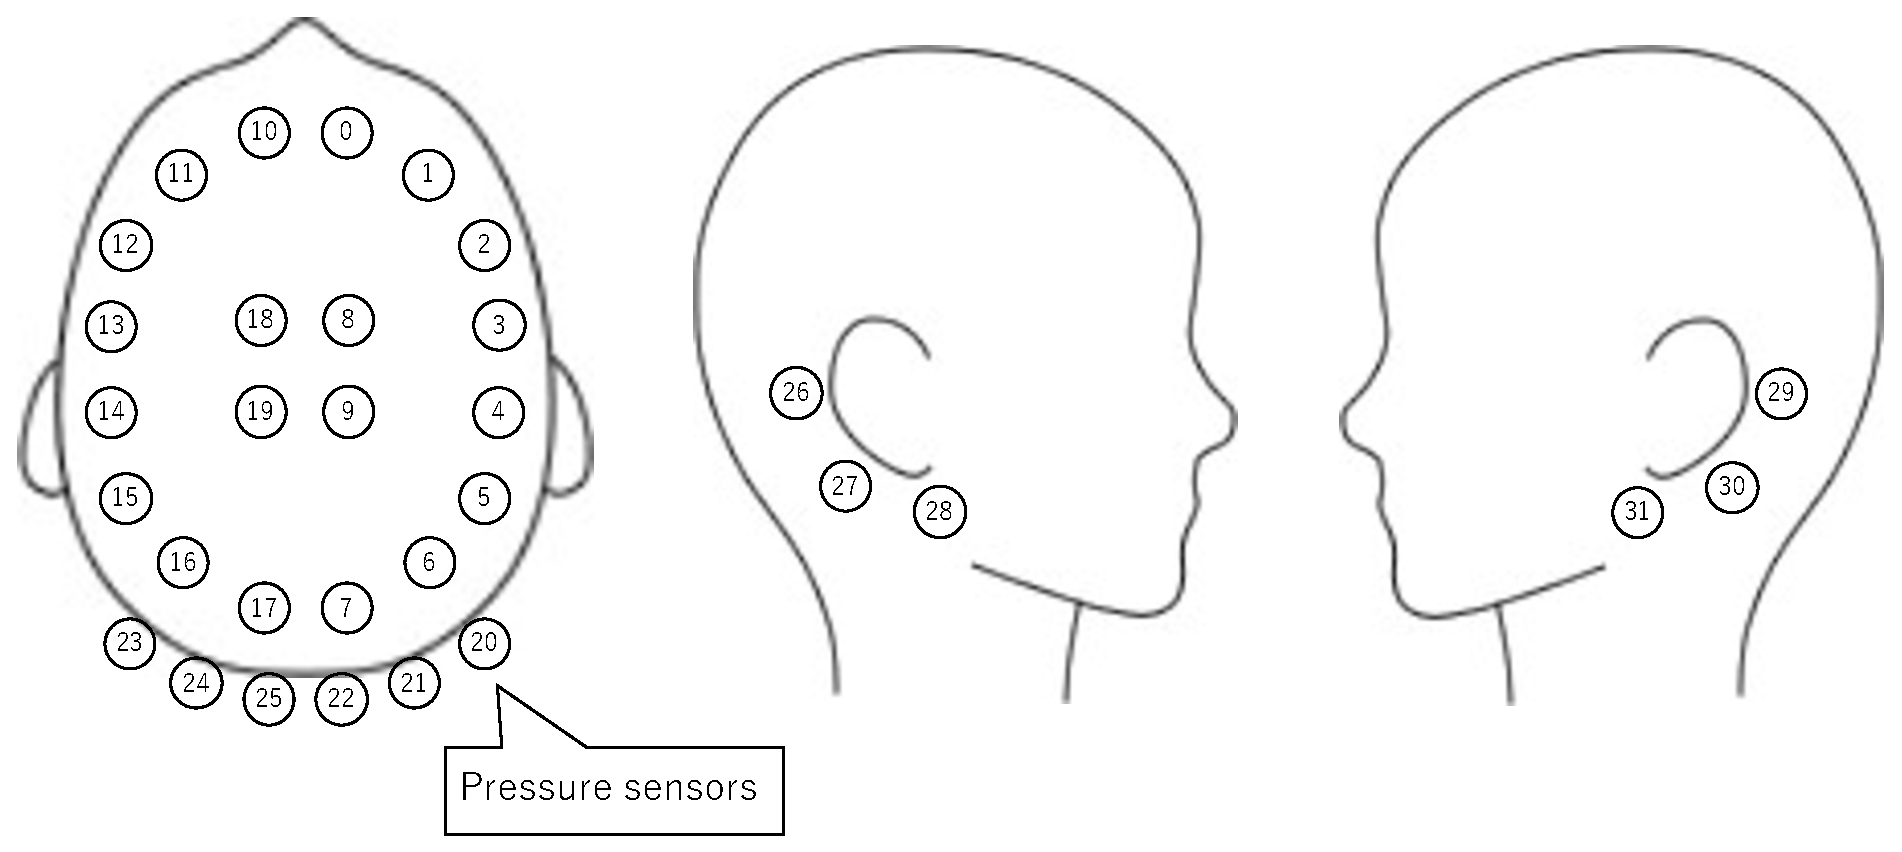
\includegraphics[width=1\textwidth]{Figure_1.eps}
%     \caption{}
%     \label{fig}
%   \end{center}
% \end{figure*}

\end{document}
